\chapter{Implementierung}\label{ch:implementierung}
Das folgende Kapitel beschreibt die Entwicklung einer Indexstruktur zur Optimierung der \textit{k}-Nächste-Nachbarn-Suche in AMBIENCE. Sie heißt \textit{BloomFilterTree}. Abschnitt \ref{sec:aufbau} beschreibt den konzeptionellen Aufbau. Die praktische Umsetzung wird in Abschnitt\ref{sec:umsetzung} dargestellt. Die zentralen Operationen Einfügen von Bloom-Filtern und \textit{k}-Nächste-Nachbarn-Suche werden in den Abschnitten \ref{sec:einfügen} und \ref{sec:knn} erläutert. Abschließend wird dargestellt, welche alternativen Ansätze während der Implementierung verfolgt und weshalb sie letztlich verworfen wurden (Abschnitt \ref{sec:alternativen}). Evaluation des Verfahrens und Gegenüberstellung mit der naiven Implementierung finden sich im folgenden Kapitel \ref{ch:evaluation}.  
\section{BloomFilterTree}\label{sec:bloom-filter-tree}
Um möglichst plattformunabhängig zu bleiben, wurde die Implementierung in C++ realisiert. Ausgewählte Codebeispiele finden sich im Anhang (vgl. Kapitel \ref{ch:anhang}). Zunächst war überlegt worden, teilweise auf bestehende Bibliotheken für Bloom-Filter und Baumstrukturen zurückzugreifen wie die bekannte \textit{Open Bloom Filter}-Bibliothek von Arash Partow\footnote{Vgl. \url{https://github.com/ArashPartow/bloom} für den Quellcode.}. Darauf wurde schließlich aus zwei Gründen verzichtet: Einerseits liegt der Fokus der Arbeit nicht auf der Implementierung von Bloom-Filtern. Andererseits stünde durch die Verwendung bestehender Bibliotheken zu befürchten, dass Messergebnisse durch den Rechnenaufwand für nicht benötigte Operationen oder durch in AMBIENCE nicht vorhandene Optimierungen verfälscht würden. 

Eine Bibliothek für B$^+$-Bäume ist z.B. das \textit{STX B+ Tree package} von Timo Bingmann\footnote{Vgl. \url{https://github.com/bingmann/stx-btree} für den Quellcode.}. Wie in Abschnitt \ref{sec:bloom-index} dargestellt, sind keine Varianten von Indexstrukturen bekannt, die sich unverändert für AMBIENCE übernehmen ließen. Auch eine bestehende Bibliothek müsste also stark abgewandelt werden. Gleichzeitig könnten dieselben Verfälschungen auftreten wie bei Verwendung einer Bloom-Filter-Bibliothek. So wurde auch davon abgesehen.
\subsection{Aufbau}\label{sec:aufbau} 
Am vielversprechendsten erschien es, wie Sakuma und Sato in ihrer Arbeit über "`Structured Bloom Filters Based on Similarity"'\footnote{Vgl. \cite{Sakuma2011}.} zunächst von einem B$^+$-Baum auszugehen (vgl. Abschnitt\ref{sec:bloom-index}). Dieser wurde zuerst implementiert mit allen Eigenschaften wie in Abschnitt \ref{sec:indexstrukturen} beschrieben. Anschließend wurde er schrittweise zur Organisation der Bloom-Filter erweitert: 
\begin{enumerate}
	\item Die Datensätze sind Bloom-Filter, d.h. jedes Blatt hält \textit{n} Zeiger auf die \textit{n} Bloom-Filter-Objekte, die darin eingefügt wurden. Bloom-Filter-Objekte werden über ihre ID als Primärschlüssel identifiziert. 
	\item Jeder Baumknoten hat einen Vereinigungs-Bloom-Filter. Er wird aus dem bitweisen logischen Oder aller Filter gebildet, die in den darunter liegenden Teilbaum eingefügt wurden (vgl. Abschnitt \ref{sec:bloom-index}).
\end{enumerate}
Abb. \ref{fig:pic6} veranschaulicht den Aufbau eines BloomFilterTree. Die Baumknoten sind blau markiert. Sie enhalten die Primärschlüssel der Bloom-Filter sowie Zeiger auf die Kind- bzw. Nachbarknoten. Jeder Knoten hat einen weiß markierten Vereinigungsfilter. Die violett markierten Filter repräsentieren die tatsächlichen Datensätze. Die Blätter verweisen jeweils auf die darin eingefügten Filter.
\begin{figure}[hpbt]
  \centering
  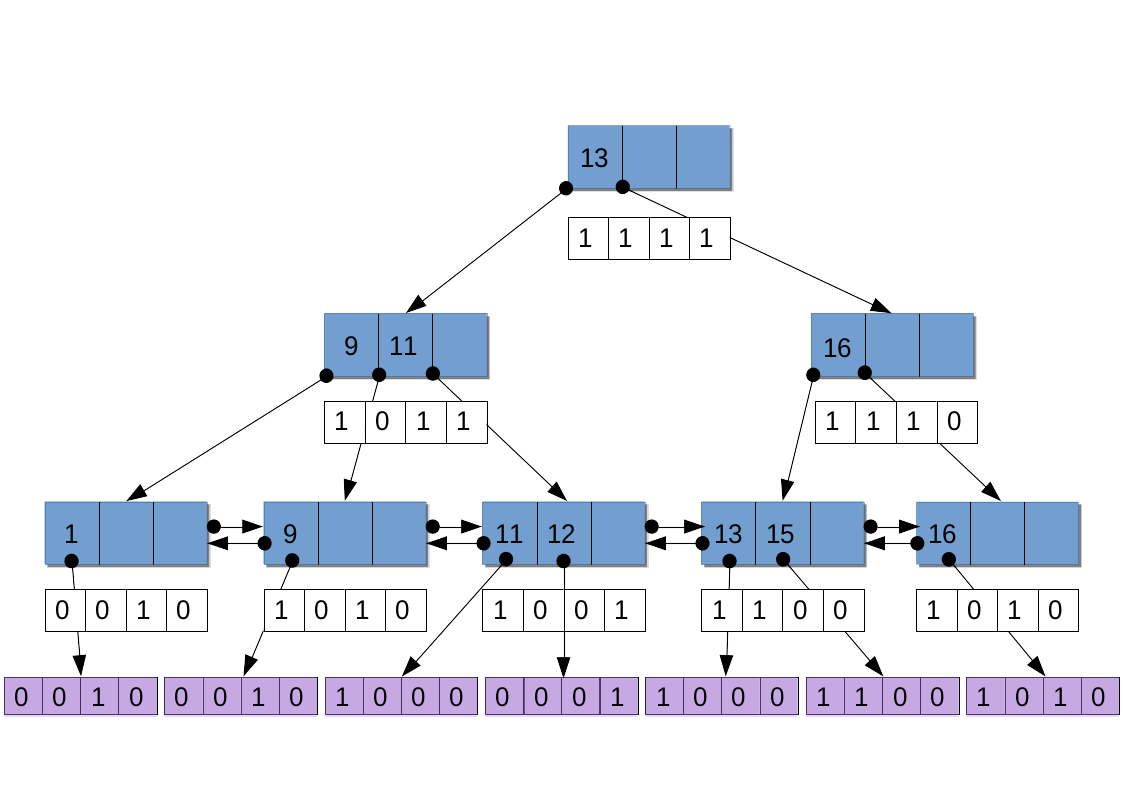
\includegraphics[width=1.0\textwidth]{pictures/bloom-filter-tree.png}\\
  \caption[Aufbau eines BloomFilterTree]{Aufbau eines BloomFilterTree mit Bloom-Filtern als Datensätzen und Vereinigungsfiltern an allen Knoten.}\label{fig:pic6}
\end{figure}
\subsection{Umsetzung}\label{sec:umsetzung}
Die Klasse \texttt{BloomFilterTree} enthält schließlich alle notwendigen Parameter und Operationen zur Organisation der Bloom-Filter. Dazu gehören die B$^+$-Baum-Operationen wie Einfügen und Suchen von Schlüsseln, Traversieren der Blätter, boolesche Abfrage nach Enthaltensein eines Schlüssel im Baum, Zählen der Blätter etc.. Darüber hinaus gibt es viele weitere Operationen: 
\begin{enumerate}
	\item \textit{Management-Operationen} zum Berechnen der Jaccard-Distanzen zu allen Filtern im Baum, naive Version der \textit{k}-Nächste-Nachbarn-Suche, Traversieren der Datensätze etc..
	\item Die \textit{zentralen Operationen} des Verfahrens: Einfügen der Bloom-Filter nach Ähnlichkeit und \textit{k}-Nächste-Nachbarn-Suche. 
	\item \textit{Mess- und Vergleichsoperationen}, um z.B. Varianten der \textit{k}-Nächste-Nachbarn-Suche, Aufbaukosten und Speicherbedarf der Datenstrukturen zu vergleichen. 
\end{enumerate}
Die Header-Datei der Klasse \texttt{BloomFilterTree} ist im Anhang abgedruckt (vgl. Abschnitt \ref{sec:BloomFilterTree.hpp}). In der Klasse \texttt{BloomFilter} wurden alle Parameter und Operationen auf Bloom-Filtern realisiert, die sich im Laufe der Arbeit als wichtig erwiesen. Dazu gehören: 
\begin{enumerate}
	\item \textit{Typische Bloom-Filter-Parameter und -Operationen:} Anzahl der Hashfunktionen, Daten-Array, Setzen von Bitpositionen etc..
	\item \textit{Mathematische und Vergleichsoperationen} wie Berechnung von Teil- und Obermengen, bitweises logisches Und und Oder, Berechnung und Abschätzung von Jaccard-Distanzen.
	\item \textit{Operationen zum Bloom-Filter-Management} wie Einfügen von zufälligen Elementen aus einem Wörterbuch oder zufällige Initialisisierung mit Werten aus $\{0,1\}$.
\end{enumerate}
Die Header-Datei der Klasse \texttt{BloomFilter} findet sich ebenfalls im Anhang (vgl. Abschnitt \ref{sec:BloomFilter.hpp}).
\subsection{Einfügen}\label{sec:einfügen}
Die Einfüge-Operation zählt zu den wichtigsten Funktionen der Indexstruktur. Sie ist entscheidend für die Optimierung von Laufzeit und CPU-Zeit der \textit{k}-Nächste-Nachbarn-Suche. Der Algorithmus basiert auf den Teil- und Obermengenbeziehungen zwischen Bloom-Filtern. Er verwendet die Vereinigungsfilter der bereits existierenden Knoten, um die optimale Position für den neu einzufügenden Filter zu finden. Falls der Baum noch leer ist, wird ein neuer Blattknoten erstellt und der Filter als erstes Datenobjekt dort eingefügt. Der neue Knoten wird zur Wurzel des BloomFilterTree. Andernfalls wird ausgehend vom Wurzelknoten rekursiv die optimale Position im Baum gesucht. Dazu werden optimale Teil- und Obermengen-IDs des Filters berechnet. Dem Filter wird die neue Teilmengen-ID zugewiesen und er wird gemäß der B$^+$-Baum-Regeln in den Baum eingefügt. Sind Teilmengen- und Obermengen-IDs unterschiedlich, wird ein zweites Datenobjekt mit der Obermengen-ID erstellt und ebenfalls in den Baum eingefügt. Falls der Baum während des Einfügens eine neue Ebene erhalten hat, wird der Elternknoten des alten Wurzelknoten zur neuen Wurzel. Abbildung \ref{fig:pic7} verdeutlicht den Ablauf:  
%\begin{figure}[hpbt]
%  \centering
%  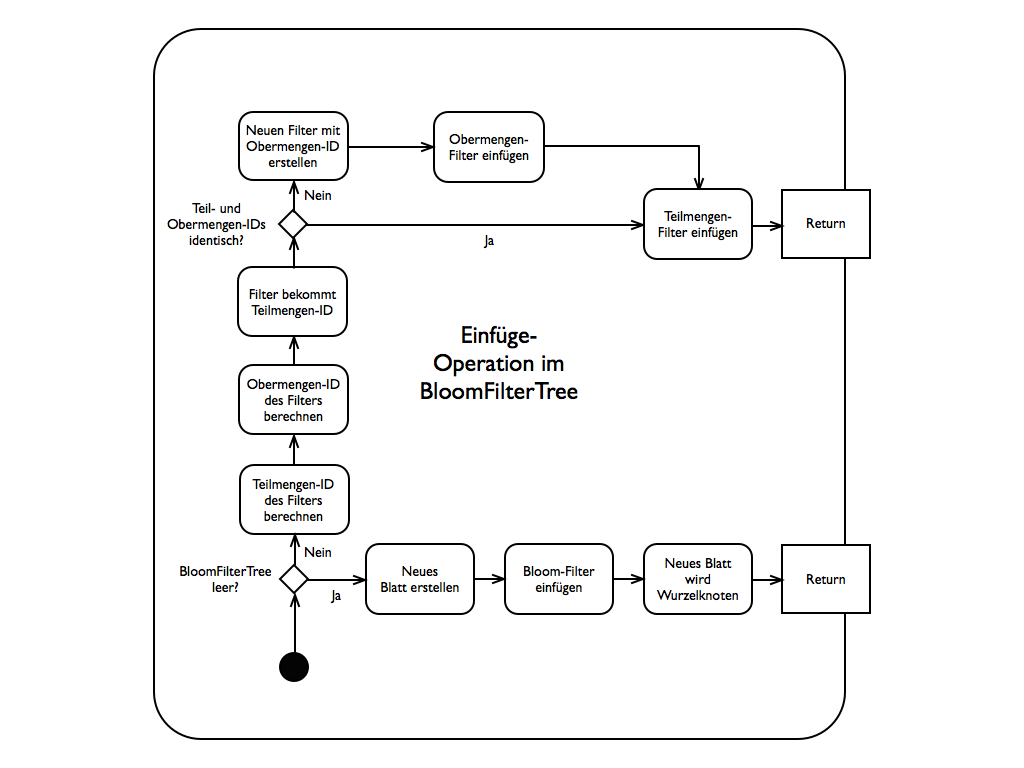
\includegraphics[width=0.9\textwidth]{pictures/insert-as-sets.png}\\
%  \caption[Einfügen von Objekten im BloomFilterTree]{Einfügen von Objekten im BloomFilterTree.}\label{fig:pic7}
%\end{figure}
Die Hauptarbeit des Einfügens findet in den Blattknoten statt, wo die Teilmengen- und Obermengen-IDs der Filter berechnet werden. Zur Berechnung der Teil\-mengen-ID werden folgende Schritte ausgeführt: 
\begin{enumerate}
	\item Einsammeln aller Bloom-Filter-Objekte im Baum, von denen der einzufügende Filter eine Teilmenge ist.
	\item Sortieren der gesammelten Filter nach Jaccard-Distanz in aufsteigender Reihenfolge.
	\item Einsammeln aller freien IDs im Baum zwischen der kleinsten und größten ID. 
	\item Sortieren der freien IDs in aufsteigender Reihenfolge.
	\item Falls der Filter von keinem Objekt im Baum eine Teilmenge ist, wird die kleinste freie ID zurückgegeben. 
	\item Andernfalls wird die optimale Teilmengen-ID bestimmt. Dazu werden zu allen in Schritt 2 gesammelten Filtern jeweils die nächstgrößere und nächstkleinere freie ID bestimmt. Diese "`guten"' IDs werden in einem Vektor gesammelt. 
	\item Die "`guten"' IDs werden nach Distanz zu einem Teilmengen-Filter des Anfragefilters sortiert. 
	\item Die ID mit der kleinsten Distanz zu einem Filter, von der der neu einzufügende Filter eine Teilmenge ist, wird als Ergebnis zurückgegeben. 
\end{enumerate}
Die Funktion \texttt{computeSubsetId()} ist beispielhaft im Anhang abgedruckt (vgl. Abschnitt \ref{sec:computeSubsetId()}). Die Berechnung der optimalen Obermengen-ID geschieht analog dazu in der Funktion \texttt{computeSupersetId()}, nur dass dazu die Obermengen des neuen Filters betrachtet werden. 
\subsection{\textit{k}-Nächste-Nachbarn-Suche}\label{sec:knn}
Das eben beschriebene Verfahren zum Einfügen von Objekten ist wesentlich aufwändiger als normalerweise beim B$^+$-Baum. Die Berechnung der optimalen Teil- und Obermengen-IDs für einen neuen Filter dient dazu, Filter mit bestehenden Teil- und Obermengenbeziehungen nahe beieinander im Baum abzuspeichern. Die \textit{k}-Nächste-Nachbarn-Suche musste natürlich darauf abgestimmt werden. Sie vergleicht nicht wie in der naiven Implementierung \textit{k}-mal die Distanzen aller Bloom-Filter im Baum zum Anfragefilter und gibt die Filter mit den \textit{k} kleinsten Distanzen zurück. Stattdessen werden die Vereinigungsfilter der Baumknoten danach untersucht, ob sie zum Anfragefilter in Teil- oder Obermengenbeziehung stehen. Ziel ist es, bei einer Anfrage nur den besten Zweig im Baum zu verfolgen.

Wie im vorigen Abschnitt dargestellt, werden die Filter beim Einfügen nach Teil- und Obermengenbeziehungen angeordnet. Der Vereinigungsfilter jedes Baumknotens enthält die Vereinigungsmenge aller Filter in seinem Teilbaum. Damit lässt sich die \textit{k}-Nächste-Nachbarn-Suche deutlich verkürzen. 

Da die \textit{k}-Nächste-Nachbarn-Suche teurer und aufwändiger ist als eine Punktanfrage nach einem Objekt, wurden dafür zwei verschiedene Operationen implementiert. Die Punktanfrage geschieht in folgenden Schritten: 
\begin{enumerate}
	\item Falls der Baum leer ist, wird der Zeiger auf den Anfragefilter selbst zurückgegeben. 
	\item Andernfalls wird geprüft, ob der Wurzelknoten Teil- oder Obermenge des Anfragefilters ist. 
	\item Ist das nicht der Fall, wird eine normale Nächste-Nachbarn-Suche auf dem Baum ausgeführt. 
	\item Andernfalls wird rekursiv beim Wurzelknoten beginnend geprüft, welche Vereinigungsfilter der Kindknoten Teil- oder Obermengen des Anfragefilters sind. 
	\item Gibt es mehrere davon, wird der Kindknoten mit der kleinsten Jaccard-Distanz des Vereinigungsfilters zum Anfragefilter bestimmt. Nur dieser Pfad wird weiter verfolgt.
	\item Gibt es keine Teil Teil- oder Obermengenbeziehungen zu den Vereinigungsfiltern der Kindknoten, wird eine Nächste-Nachbarn-Suche auf dem restlichen Teilbaum durchgeführt. 
	\item Ist die Anfrage auf der Blattebene angekommen, wird der Filter mit der kleinsten Distanz im Blatt bestimmt und ein Zeiger darauf zurückgegeben.  
\end{enumerate}
Auch wenn ab einem bestimmten Punkt keine Teil- oder Obermengenbeziehungen mehr zwischen Anfragefilter und den Vereinigungsfiltern der Kindnoten des aktuellen Knoten bestehen, wird die Anfrage deutlich abgekürzt. Dann muss nur noch eine Nächste-Nachbarn-Suche auf einem Teilbaum durchgeführt werden, nicht auf der gesamten Indexstruktur. 

Hier findet offensichtlich die hauptsächliche Arbeit in den inneren Knoten des BloomFilterTree statt, den so genannten Index- oder Directoryknoten. Bei der\textit{k}-Nächste-Nachbarn-Suche findet hingegen wie zuvor ein großer Teil der Sortierarbeit auf Blattebene statt. Abbildung \ref{fig:pic8} zeigt den Ablauf im BloomFilterTree: 
%\begin{figure}[hpbt]
%  \centering
%  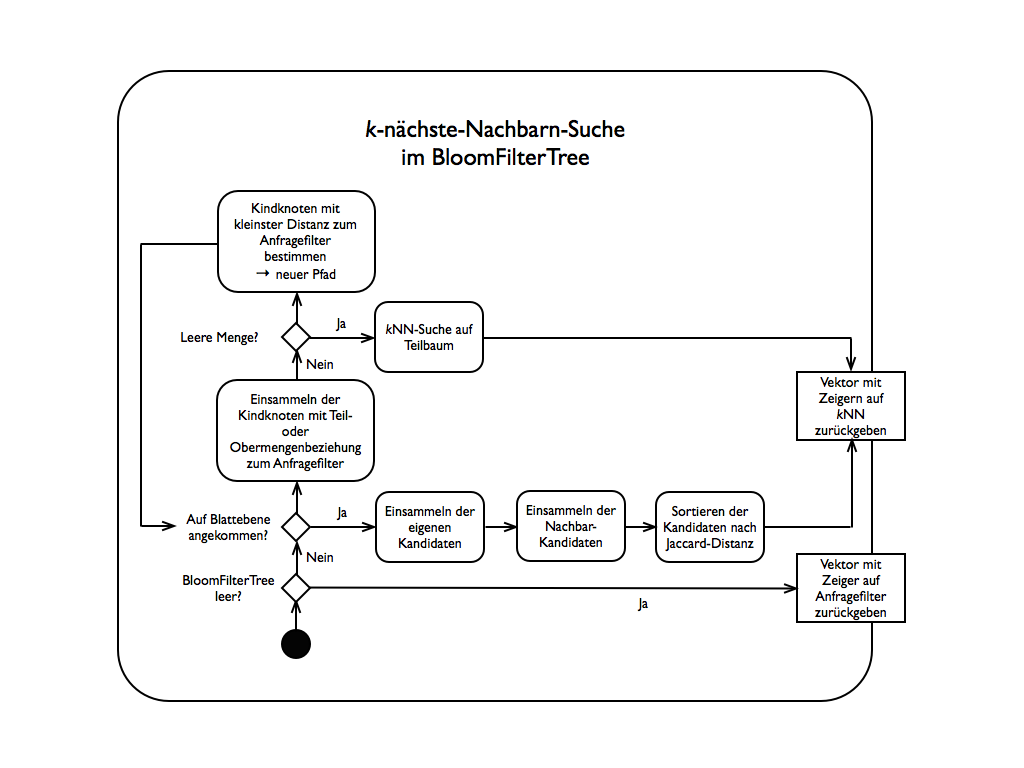
\includegraphics[width=0.9\textwidth]{pictures/knn.png}\\
%  \caption[\textit{k}-Nächste-Nachbarn-Suche im BloomFilterTree]{\textit{k}-Nächste-Nachbarn-Suche im BloomFilterTree.}\label{fig:pic8}
%\end{figure}
Die Quellcode der Funktion \texttt{simQueryVec()} der Klasse \texttt{BloomFilterTree} ist beispielhaft im Anhang abgedruckt (vgl. \ref{sec:simQueryVec()}). Wie die Evaluation in Kapitel \ref{ch:evaluation} zeigt, lassen sich mit den vorgestellten Methoden Laufzeit und CPU-Zeit der k-Nächste-Nachbarn-Suche deutlich reduzieren. 

Ergänzend lässt sich anmerken, dass bei allen vorgestellten Funktionen die B$^+$-Baum-spezifische Bereichssuche von Nutzen ist. Die komplexe Einfüge-Operation wurde dadurch erleichtert, dass z.B. zum Einsammeln aller freien IDs nur einmal die Blattebene traversiert werden muss. Andere Baumstrukturen benötigen dazu in der Regel eine deutlich komplexere Breiten- oder Tiefensuche. Bei der \textit{k}-Nächste-Nachbarn-Suche in einem Teilbaum muss ebenfalls nur der Teilbereich zwischen einem Start- und Endwert traversiert werden. Das liegt daran, dass die Blätter eine doppelt verkettete Liste bilden und die Indexstruktur die Suchbaumeigenschaft auf den Primärschlüsseln, d.h. den Bloom-Filter-IDs, erfüllt.  
\section{Alternative Ansätze}\label{sec:alternativen}
Zum Abschluss des Kapitels werden zwei Ansätze vorgestellt, die alternativ zum BloomFilterTree bzw. zur Organisation nach Teil- und Obermengenbeziehungen verfolgt wurden. Letztlich erwies sich die Kombination aus Baumstruktur und Mengenbeziehungen am erfolgreichsten, der Vollständigkeit halber werden sie trotzdem kurz präsentiert. 
\subsection{Einfügen gemäß Jaccard-Distanzen}\label{sec:ähnlichkeit}
Anfangs wurde der Ansatz verfolgt, die Bloom-Filter analog zur Arbeit von Sakuma und Sato an Hand ihrer Distanzen im Baum zu organisieren (vgl. Abschnitt \ref{sec:bloom-index}). An diesem Punkt stellte sich heraus, dass das dort verwendete Distanzmaß transitiv ist im Sinne von Abschnitt \ref{sec:distanzmasse}. Das trifft auf die Jaccard-Distanz nicht zu. Die Suche nach Alternativen ergab die Kombination aus Vereinigungsfilter und Transitivität der Teil- und Obermengenbeziehungen, die letztlich umgesetzt wurde. 
\subsection{Doppelt verkettete Liste}\label{sec:verkettete-liste}
Eine andere Idee war die Gruppierung der Filter nach Gleichheit von Teilsegmenten. Als Datenstruktur sollte eine doppelt verkettete Liste dienen mit derselben Anzahl an Listenknoten wie Positionen im Bloom-Filter. Die einzufügenden Bloom-Filter wurden in Segmente unterteilt. Ein Segment entsprach dabei einem Element im Daten-Array. Ein neuer Filter wurde wie folgt in die Datenstruktur eingefügt:  
\begin{enumerate}
	\item Jeder Listenknoten hat eine 0- und eine 1-Bit-Liste. Darin sind Zeiger auf die bereits eingefügten Filter gespeichert, die an derselben Bitposition eine 0 bzw. eine 1 enthalten. 
	\item Wird ein neues Objekt in die Liste eingefügt, wird an jedem Listenknoten die entsprechende Liste aktualisiert, je nachdem, ob der einzufügende Filter an der Position 0 oder 1 enthält. 
\end{enumerate}
Das Ziel war, bei der \textit{k}-Nächsten-Nachbarn-Suche die 0- bzw. 1-Bit-Listen der Listenknoten mit gleichem Segmentinhalt abzuprüfen. Alle darin enthaltenen Zeiger wurden in einem Vektor gesammelt, der nach Häufigkeit der Zeiger sortiert wurde. Es bestand die Hoffnung, dass sich die am häufigsten vorkommenden Zeigern und die nächsten Nachbarn des Anfragefilters proportional zueinander verhielten.
 
Eine solche Datenstruktur ist in Implementierung und Pflege weit weniger aufwändig als eine Baumstruktur. Es zeigte sich jedoch, dass damit nicht die gewünschten Ergebnisse erzielt werden konnten, da bei der \textit{k}-Nächsten-Nachbarn-Suche zu viele Ergebnisse mit gleich vielen Zeigern gefunden wurden. Die Suche scheiterte somit an mangelnder Ergebnisqualität und die doppelt verkettete Liste wurde als Datenstruktur verworfen. 